\chapter{防火墙}
%\clearquestion
\question{什么是防火墙}
防火墙是一种协助确保信息安全的设施,\textbf{依照特定的规则},允许或是禁止传输的数据通过。

\question{防火墙放置位置}
位于信任内部网络和不可信任的外界网络之间,如网关,防火墙主机上的一些特定的应用程序。

\question{防火墙的特性}
\begin{enumerate}
	\item 内部网络和外部网络之间的所有网络数据都必须经过防火墙
	\item 只有符合安全策略的数据流才能通过防火墙
	\item 防火墙自身应具有非常强的抗攻击免疫力
\end{enumerate}

\question{防火墙的功能}
\begin{enumerate}
	\item 防火墙是网络安全的屏障
	\item 防火墙可以强化网络安全策略
	\item 防火墙可以对网络存取和访问进行监控审计
	\item 防火墙可以防范内部消息的外泄
\end{enumerate}

\question{防火墙网络层的性质指标}
\begin{enumerate}
	\item 吞吐量指标
	\item 时延指标
	\item 丢包率指标
	\item 背靠背缓冲指标
\end{enumerate}

\question{防火墙常见的功能指标}
\begin{enumerate}
	\item 服务平台支持
	\item LAN口支持
	\item 协议支持
	\item VPN支持
	\item \dots
\end{enumerate}

\question{防火墙核心技术}
\begin{enumerate}
	\item 包过滤技术,在\textbf{网络层}截获网络数据包,根据防火墙的规则表,来检测攻击行为,在网络层提供较低级别的安全防护和控制
	\item 应用网关技术,又被成为代理技术,位于应用层上,所以主要采用协议代理服务。应用代理防火墙壁分组过滤防火墙提供更高层次的安全性,但这丧失对应用程序的透明性。
	\item 状态检测技术,采用一种基于连接的状态监测机制,将属于同一连接的所有包作为一个整体的数据流看待,构成连接状态表,通过规则表与状态的共同配置,对表中的各个连接状态因素加以识别。\textbf{是一种动态的判定方法。(前两种为静态)}Steps:
	\begin{itemize}
		\item 检查是否属于一个已建立的连接
		\item 若已建立,则根据连接状态表的策略对数据包实施丢弃、拒绝或是转发。
		\item 若未建立连接,会检查数据包是否与他配置的规则集匹配。
	\end{itemize}
\end{enumerate}

\question{防火墙分类}
\begin{enumerate}
	\item 个人防火墙
	\item 分布式防火墙
	\item 分层式防火墙
\end{enumerate}

\question{防火墙的体系结构,部署位置}
\hspace{2em}\\
基本概念:
\begin{enumerate}
	\item 堡垒主机,一种被强化的可以防御攻击的计算机,作为进入内部网络的一个检查点。堡垒主机是网络中\textbf{最容易受到侵害}的主机。\textbf{包过滤路由器和应用代理服务器均可视为堡垒主机。}
	\item 非军事区,也成为“隔离区”,他是为了解决安装防火墙后,外部网络不能访问内部网络服务器的问题,而设立的一个非安全系统与安全系统之间的缓冲区。
\end{enumerate}
体系结构分类:
\begin{enumerate}
	\item 筛选路由器体系结构。
	\item 单宿主堡垒主机,由包过滤路由器和堡垒主机构成。外部路由器配置把所有进来的数据发送到堡垒主机上,所有出去的数据包也经过堡垒主机(代理)。实现了网络层安全(包过滤)和应用层安全(代理服务)。缺点:可通过重新配置路由器,使数据绕过堡垒主机。
	\item 双宿主堡垒主机,与单宿主堡垒主机的区别在于,双宿主堡垒主机有两块网卡,一块连接内部网络,一块连接包过滤路由器,但是主机两个端口之间直接转发信息的功能被关闭。在应用层提供代理服务
	\item 屏蔽子网体系结构:由两个包过滤路由器和一个堡垒主机构成,支持网络层和应用层的安全功能。在定义非军事区(DMZ),即屏蔽子网后。存在内部防火墙和外部防火墙。攻击者要通过外部防火墙,堡垒主机和内部防火墙三道防线,才能到达内部网络。
	\begin{figure}[H]
		\centering
		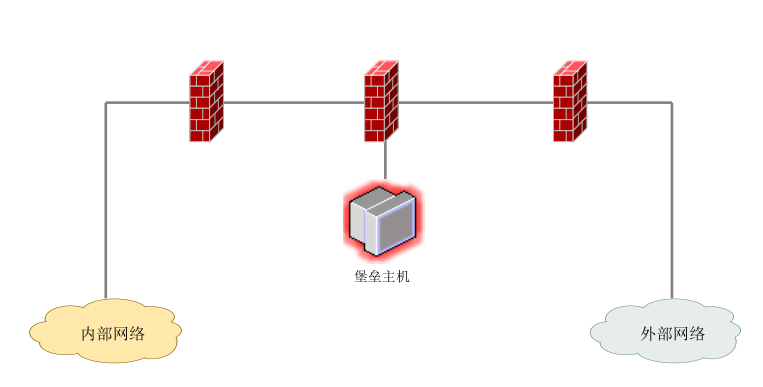
\includegraphics[width=0.7\linewidth]{figures/screenshot001}
		\caption{}
		\label{fig:screenshot001}
	\end{figure}
\end{enumerate}

\question{常见产品}
\begin{enumerate}
	\item Firewall
	\item PIX
	\item AXENT Raptor
	\item NetScreen
	\item 天融信网络卫士
	\item 东软NetEye  4032防火墙
\end{enumerate}





